\chapter{Evaluation}\label{ch:evaluation}
Our evaluation answers the following questions.
(i) How well does {\sys} mitigate state-of-the-art network side-channel attacks?
(ii) What are the overheads associated with varying DP configuration parameters?
(iii) What are {\sys}'s overall costs on privacy and bandwidth for different classes of applications?
(iv) How do {\sys}'s privacy guarantees and performance overheads compare to prior techniques?


For our experiments, we use a AMD Ryzen 7 7700X desktop with eight 4.5 GHz CPUs, 32 GB RAM, 1 TB storage, and a GTX 4090 GPU.
We use two applications as case studies, a video streaming service and a medical web service, which we describe below.
From each application, we collect two different sets of traces to evaluate the privacy and overhead of our shaping mechanism.
\paragraph{Video service.}
The video streaming service is hosted on an Nginx 1.23.4 web server and is used to serve 100 YouTube videos in 720p resolution.
The videos are stored on a standard file system on the host OS and have durations ranging from 5 min to 130.3 min (median 12.6 min) and sizes ranging from 2.7 MB to 1.4 GB (median 73.7 MB).
We stream the first 5 minutes of each video 100 times and collect the traces, leading to 10000 traces in total.

\paragraph{Web service.}
The web service is also hosted on Nginx 1.23.4 and is used to serve a corpus of 100 static HTML pages of a medical website.
The web pages are stored on a standard file system on the host OS and have sizes ranging from 54 KB to 147 KB (median: 90 KB).
Similar to the video dataset, we request each webpage 100 times, resulting in a dataset with 10000 traces in total.
%


In \Cref{sec:eval-tcn}, we provide a brief overview of our TCN-based video identification attack, where we use temporal neural networks (TCN) to map the pattern of the traffic trace to its content.
Then, in \Cref{sec:eval-empirical-privacy} we use our TCN-based video identification attack to evaluate the privacy of DP traffic shaping empirically.
In \Cref{sec:eval-privacy-params}, we measure the effect of various parameters in our system on the privacy loss associated with our DP shaping mechanism. 
In \Cref{sec:eval-bw}, we measure the bandwidth and latency overheads of DP shaping mechanism with two different application: video streaming and web services.
Finally, we compare overheads of {\sys} with other traffic shaping techniques.  


\section{TCN-based Video Identification}\label{sec:eval-tcn}

Beauty and the Burst~\cite{schuster2017beautyburst} uses Convolutional Neural Networks (CNNs) for video identification. 
CNNs have been shown to be effective in sequence modeling for decades~\cite{hinton1990connectionist}.
However, there are two problems with using a convolutional neural network as a sequence modeler.
First, convolutional layers applied to a sequence are not inherently causal, meaning that they look into future samples of a sequence to decide the output for the current sample.
Secondly, convolutional neural networks lack a deep effective history size of past samples in the sequence (i.e. their effective history is bounded to the number of samples that kernel can cover from the past).
To address these problems, Bai\etalc{bai2018empirical} proposed a new architecture called Temporal Convolutional Network (TCN).
The TCN utilizes a one-dimensional fully-convolutional network~\cite{long2015fully} equipped with causal dilated convolutions~\cite{oord2016wavenet}, allowing it to examine deep into the past to produce an output for the sequence at any given moment.
They added a generic residual block from input to output.
The architecture is shown in the \Cref{fig:tcn-arch}.
We evaluate the effectiveness of TCN model for network side-channel attacks in \Cref{sec:eval-empirical-privacy}.



\begin{figure}[t]
  \centering
  %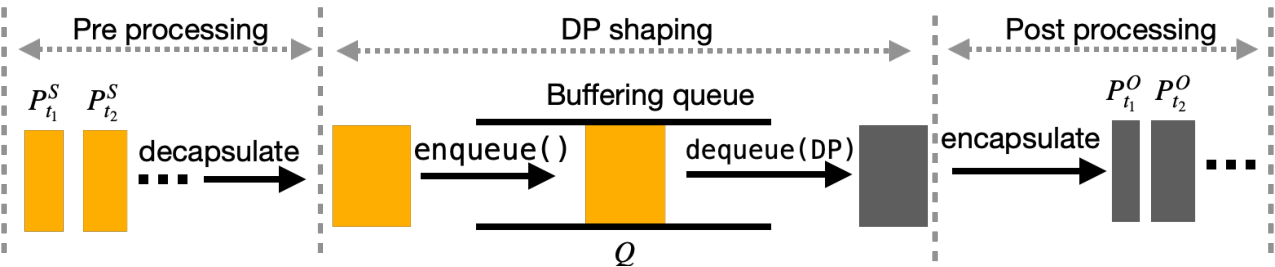
\includegraphics[width=\columnwidth]{figures/DPshaping_concept_vertical.pdf}
  %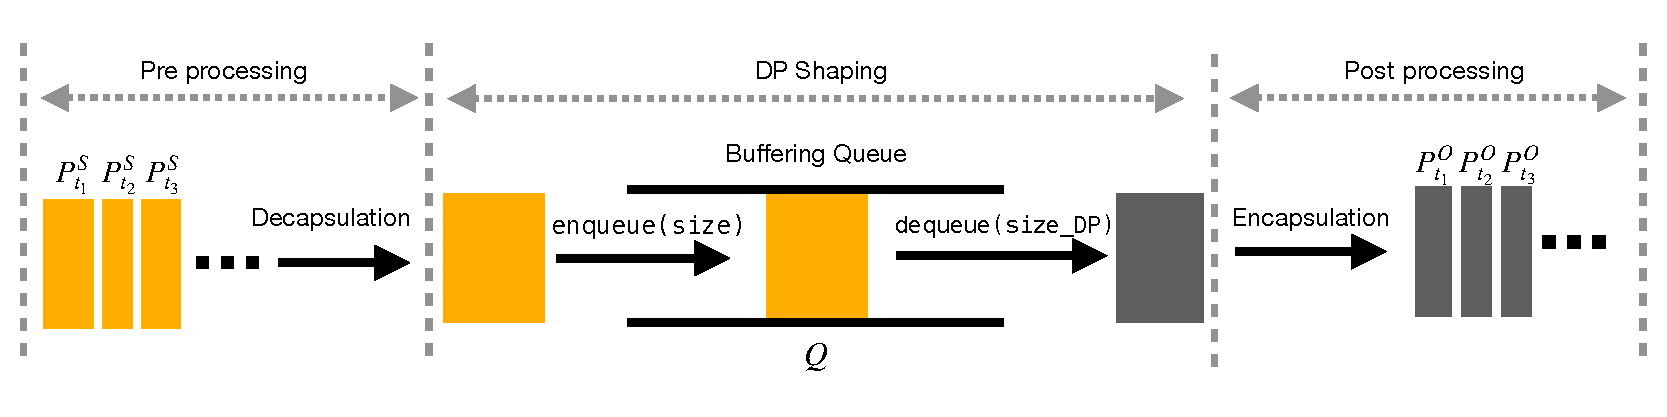
\includegraphics[width=\columnwidth]{figures/DPshaping_concept_horizontal.pdf}
  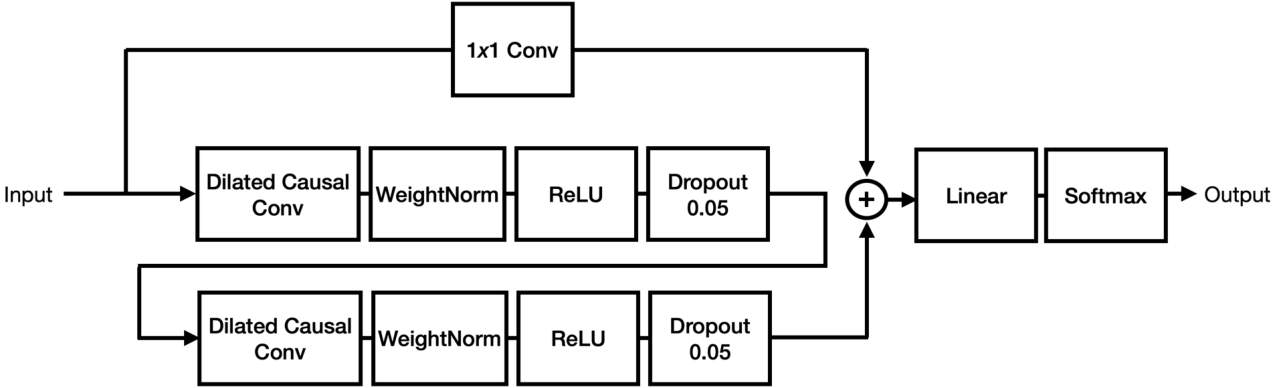
\includegraphics[width=\columnwidth]{figures/TCN_arch.pdf}
  \caption{TCN model architecture.}
  \label{fig:tcn-arch}
\end{figure}



\section{Empirical Privacy Evaluation}\label{sec:eval-empirical-privacy}
We start with an empirical evaluation of the privacy offered by {\sys}'s traffic
shaping.
To evaluate privacy empirically, we first establish the baseline for comparison, which is attacker accuracy, precision, and recall on unmodified (\ie unshaped) traces.
We set up the video service and a video client as two Amazon AWS VMs placed in Oregon and Montreal, respectively.
The client streams the first 5 min of all videos of our video dataset over HTTPS and collects the resulting network packet traces using tcpdump.
We also filter our dataset comprising 10,000 traces and 100 videos to reduce it to a smaller dataset consisting of 40 videos and 4,000 traces.
We evaluate the Beauty and the Burst (BB) model and our TCN-based model with the collected traces using both small and large datasets.
The objective of the models is to determine the corresponding video title for a given trace. 
For each model, we transform each packet trace into a sequence of burst sizes
transmitted within 1s windows.
Therefore, the input to the classifier is a time series representing burst sizes with burst length of 1 second.
We normalize the time series by dividing each burst size by the total size of the corresponding trace.
For each dataset, we use 80\% of traces to train the model and 20\% of traces to test it. 
We train both models for 1000 epochs\footnote{An epoch refers to one complete pass through the entire training dataset during the training.} and report the accuracy, precision, and recall on the test data.
\Cref{tab:attack-performance} represents the result for both models with the two datasets.
Our TCN model outperformes BB model on both datasets. 
Specifically, BB struggles with the larger dataset and its accuracy drops to random guess. 
The presence of residual layers in TCN makes it a better choice for a larger dataset.
\begin{table}[h]
  \centering
  \caption{Attack Performance on unshaped traffic}
  \begin{tabular}{|l|c|c|c|c|}
    \hline
    \textbf{Attack} & \textbf{\# of videos} & \textbf{Accuracy} & \textbf{Precision} & \textbf{Recall} \\ 
    \hline
    \multirow{2}{*}{TCN} & 100 & 0.995 & 0.99 & 0.99 \\ 
                         & 40  & 0.996 & 0.99 & 0.99 \\ 
    \hline
    \multirow{2}{*}{BB}  & 100 & 0.005  & 0.005 & 0.01 \\ 
                         & 40  & 0.61  & 0.49 & 0.63 \\ 
    \hline
  \end{tabular}\label{tab:attack-performance}
\end{table}

Next, we evaluate the efficacy of our differentially-private shaping mechanism against both BB and TCN attacks with the small dataset.
We did not consider the large dataset for this task because the BB model failed to classify the baseline unshaped traffic, making it impossible to see the effectiveness of the DP shaping mechanism for this attack.
The performance of the DP traffic shaping depends on several parameters: the window length $\winlen$, the sensitivity for neighboring streams $\ssens$, the length of the DP measurement interval $\dpintvl$, and the privacy loss $\varepsilon_{\winlen}$.
The privacy of the mechanism, however, is characterized by the privacy loss, $\varepsilon_{\winlen}$
Therefore, we fix values of $\ssens$, $\winlen$, and $\dpintvl$ and measure the accuracy of classifier for varying values of $\varepsilon_{\winlen}$.
As both of attacks fail to perform effectively with small values of $\varepsilon_{\winlen}$ (\ie lower privacy loss), we increment $\varepsilon_{\winlen}$ until one of the attacks yields an accuracy beyond random guessing (\ie $\varepsilon_{\winlen} \in [100, 43000]$).
Our goal is to provide intuition about practical values of $\varepsilon_{\winlen}$ that are sufficient to thwart a side-channel~attack.

We set (i) $\winlen = 5s$ to align with the 5s video segments that comprise the videos, (ii) $\ssens = 1 MB$, which covers 97\% of the video streams in our dataset, and (iii) $\dpintvl = 1s$, which leads to composing the privacy loss over $\varnumupdates = 5$ DP measurements of the buffering queues.

We use 4000 traces of 40 videos, each with 5 minutes duration (\ie small dataset).
For each value of $\varepsilon_{\winlen}$, we transform each unshaped trace into a shaped trace using our simulator to generate a total of 4000 shaped traces.
We train the classifier on 3200 shaped traces and measure the accuracy of the attack model on 800 shaped traces.

\Cref{fig:empirical-privacy} shows the average (markers) and the standard deviation (shaded region) of the accuracy of each classifier over three runs on the shaped traces.
While BB does not perform well for any values of $\varepsilon_{\winlen}$, TCN can be thwarted only for $\varepsilon_{\winlen} < 1000$ with {\sys} (\ns).
The BB and TCN accuracy on unshaped traffic ({\base}) is 0.61 and 0.99, respectively (see \Cref{tab:attack-performance}).
Note that large values of privacy loss (\ie $\varepsilon_{\winlen} \leq 1$) does not provide meaningful theoretical privacy guarantees.
For example, $\varepsilon_{\winlen}=10$ means that given a trace, in the worst-case, the probability that the adversary can correctly identify the video title is $e^{10} \approx 22000$ times larger than the probability that the adversary fails to classify it correctly.
Nonetheless, in practice, we observe that small perturbations with large privacy losses are enough to thwart the state-of-the-art attacks.
This observation highlights the large gap between theoretical guarantees and empirical evaluation of side-channel attacks, which has two important implications: First, the successful mitigation of present attacks by a defense doesn't assure its efficacy against future, more sophisticated attacks.
Second, these findings encourage the development of network side-channel defense mechanisms and their subsequent evaluation based on theoretical privacy considerations, because the empirical evaluation can potentially overestimate the effectiveness of these mechanisms.


\begin{figure}[t]
  \centering
  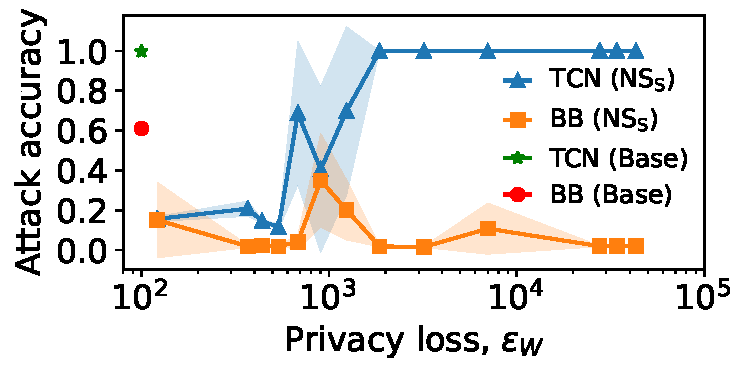
\includegraphics[width=\columnwidth]{plots/accuracy_vs_privacy_loss_video.pdf}
  \caption{Classifier accuracy on shaped traces.
      %    \am{Change label from {\ns} to {\nssim}}
  }
  %\am{How is the blue shaded area going higher than accuracy of 1.0?}\as{The
      %blue shaded area is +-std so it can be larger than one or smaller than
      %zero.}
  \label{fig:empirical-privacy}
\end{figure}

\section{Impact of Privacy Parameters}\label{sec:eval-privacy-params}
We, now,  evaluate how $\varepsilon_{\winlen}$ varies with $\sigma_\dpintvl$, $\varnumupdates$, and $\ssens$.
All analyses use $\delta_\winlen = 10^{-6}$ for two different classes of applications: applications with high sensitivity such as video streaming and applications with lower value of sensitivity such as web browsing.
The sensitivity value represents the highest potential change in the buffering queue size when two distinct traffic traces pass through the shaping mechanism.
If the change in queue size surpasses the sensitivity value, it results in a privacy loss exceeding the intended $\varepsilon_{\winlen}$ threshold.
Nevertheless, the privacy guarantees provided by Differential Privacy (DP) remain applicable even in cases where the privacy loss exceeds the sensitivity, resulting in traffic shaping with larger privacy loss values.


\Cref{subfig:high-sensitivity-epsilon-sigma} and \Cref{subfig:low-sensitivity-epsilon-sigma} show the trade-off between privacy loss ($\varepsilon_{\winlen}$) and noise ($\sigma_\dpintvl$) over four different numbers of DP measurements ($\varnumupdates$) for two different setups.
Intuitively, a larger $\sigma_\dpintvl$ implies higher bandwidth overhead due to DP shaping.
Besides that, applications with higher sensitivity, denoted as $\ssens$, particularly require larger values of $\sigma_\dpintvl$ to provide the same levels of privacy guarantees.
For example, for an application with a sensitivity of $\varepsilon_{\winlen}=1MB$, according to \Cref{subfig:low-sensitivity-epsilon-sigma}, to retain a total privacy loss $\varepsilon_{\winlen} = 1$ with at most 4 DP measurements, we need to add noise with $\sigma_\dpintvl = 6 MB$ for each DP measurement.
Meanwhile, to have the same value of privacy loss with 4 DP measurement in an application with a lower sensitivity $\varepsilon_{\winlen}$, we need to add noise with $\sigma_\dpintvl = 0.8 MB$.

The large gap between theoretical privacy guarantees and the effectiveness of the state-of-the-art attacks is also worth highlighting in this context.
For example, $\varepsilon_{\winlen} = 100$ with 4 DP measurements (the approximate configuration that defeats the classifiers in \Cref{fig:empirical-privacy}) only requires $\sigma_\dpintvl < 0.1 MB$ even for high-sensitivity applications.
However, we configure our system to provide theoretical guarantees (\ie small values of privacy loss), and discuss how to amortize bandwidth overheads using concurrent flows without increasing privacy loss in \Cref{sec:eval-bw}.

Using these plots, an application can choose suitable values of $\ssens$ and $\winlen$ to determine the trade-off between $\varepsilon_{\winlen}$ and $\delta_{\winlen}$.
For our web application serving static HTML, we recommend $\winlen = 1s$, since web page downloads in our AWS setup finished within 1s, and $\ssens = 150 KB$, which covers 95\% of the web pages in our dataset.
Similarly, In \Cref{fig:empirical-privacy}, we explain the choices for our video application.
Using $\varepsilon_{\winlen}$ and $\dpintvl$, we can further determine the aggregate privacy loss over longer traffic streams using R\'enyi-DP composition.
For instance, with $\varepsilon_{\winlen} = 1$, $\winlen = 5s$, and $\dpintvl = 1s$, the total privacy loss for a 5 min video, which generates 300 DP measurements at 1s intervals, is 8.92; the total loss for a 1 hr video is 38.8.
We emphasize that {\em $\ssens$ and $\varepsilon_\winlen$ should be selected using trade-off plots similar to \Cref{fig:privacy-microbenchmarks-low-sensitivity} and \Cref{fig:privacy-microbenchmarks-high-sensitivity} independently of the application's dataset.}
Another approach to parameter configuration within our setup involves utilizing a publicly available dataset for the same application, such as a publicly accessible video streaming dataset or web service dataset.
This allows for the independent configuration of parameters, which can then be deployed within our system, irrespective of users' traffic.




\begin{figure}[t]
  \centering
  \begin{subfigure}{0.49\columnwidth}
      \centering
      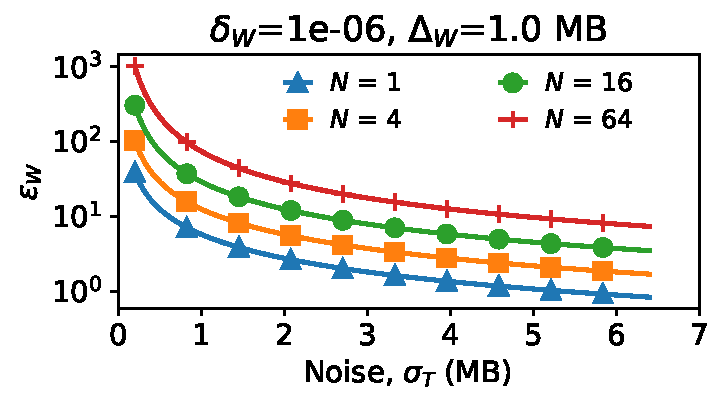
\includegraphics[width=\textwidth]{plots/privacy_loss_VS_noise_std_video.pdf}
      \caption{}
      %        \caption{Noise vs privacy loss}
      \label{subfig:high-sensitivity-epsilon-sigma}
  \end{subfigure}
  \hfill
%    \begin{subfigure}{0.33\textwidth}
  %        \centering
  %
  %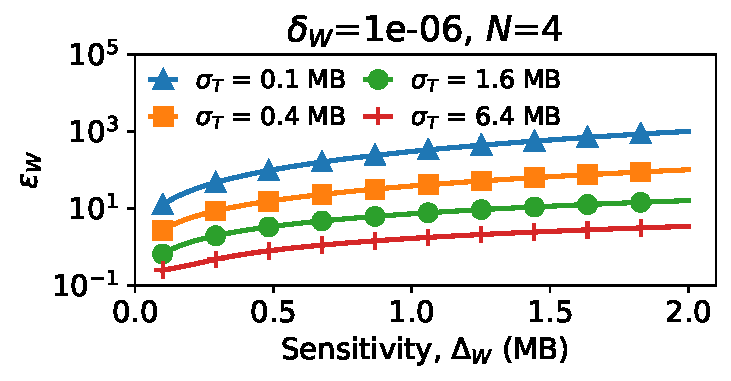
\includegraphics[width=\textwidth]{plots/privacy_loss_VS_sensitivity_video.pdf}
  %        \caption{Sensitivity vs privacy loss}
  %        \label{subfig:high-sensitivity-epsilon-sensitivity}
  %    \end{subfigure}
%    \hfill
  \begin{subfigure}{0.49\columnwidth}
      \centering
      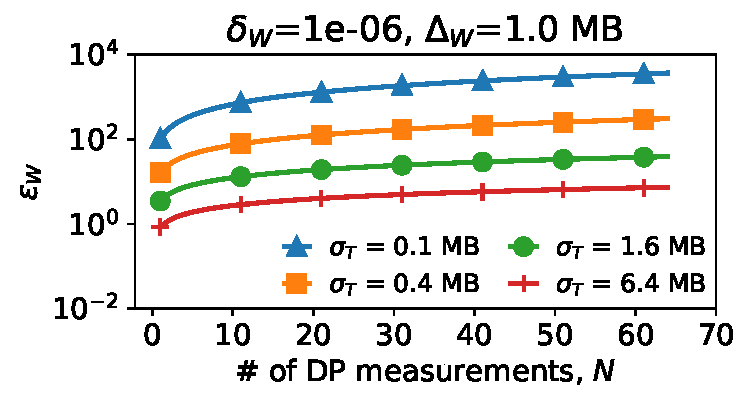
\includegraphics[width=\textwidth]{plots/privacy_loss_VS_query_num_video.pdf}
      \caption{}
%        \caption{\# of DP measurements vs privacy loss}
      \label{subfig:high-sensitivity-epsilon-queries}
  \end{subfigure}
  \caption{
    Per-window privacy loss ($\varepsilon_{\winlen}$) as a function of
    (a) noise ($\sigma_\dpintvl$), and (b) number of DP measurements ($N$).
%    \am{Make notations consistent.}
  }
  \label{fig:privacy-microbenchmarks-high-sensitivity}
\end{figure}


\begin{figure}[t]
  \centering
  \begin{subfigure}{0.49\columnwidth}
      \centering
      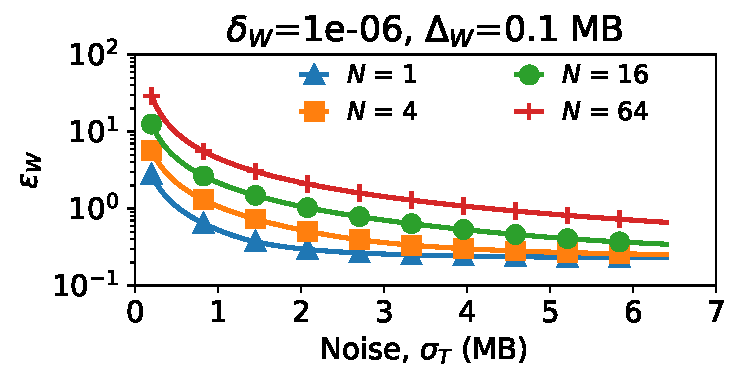
\includegraphics[width=\textwidth]{plots/privacy_loss_VS_noise_std_low_sensitivity.pdf}
      \caption{}
      %        \caption{Noise vs privacy loss}
      \label{subfig:low-sensitivity-epsilon-sigma}
  \end{subfigure}
  \hfill
%    \begin{subfigure}{0.33\textwidth}
  %        \centering
  %
  %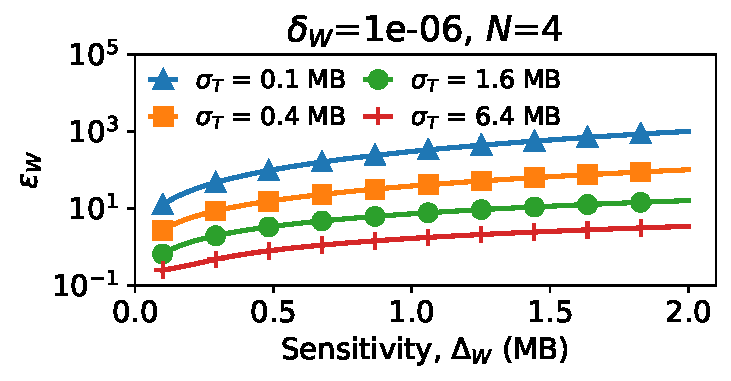
\includegraphics[width=\textwidth]{plots/privacy_loss_VS_sensitivity_video.pdf}
  %        \caption{Sensitivity vs privacy loss}
  %        \label{subfig:high-sensitivity-epsilon-sensitivity}
  %    \end{subfigure}
%    \hfill
  \begin{subfigure}{0.49\columnwidth}
      \centering
      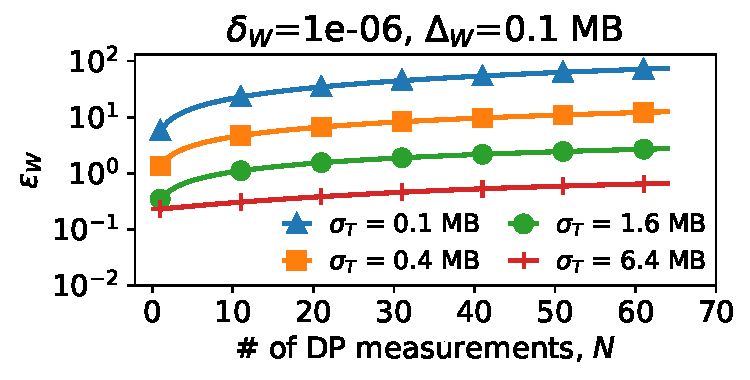
\includegraphics[width=\textwidth]{plots/privacy_loss_VS_query_num_low_sensitivity.pdf}
      \caption{}
%        \caption{\# of DP measurements vs privacy loss}
      \label{subfig:low-sensitivity-epsilon-queries}
  \end{subfigure}
  \caption{
    Per-window privacy loss ($\varepsilon_{\winlen}$) as a function of
    (a) noise ($\sigma_\dpintvl$), and (b) number of DP measurements ($N$).
%    \am{Make notations consistent.}
  }
  \label{fig:privacy-microbenchmarks-low-sensitivity}
\end{figure}

\section{DP Shaping Bandwidth and Latency Overhead}\label{sec:eval-bw}
In this section, we measure the bandwidth overheads of {\sys} for two different applications using our traffic shaping simulator (see \Cref{sec:eval-simulator}).
We present two case studies. 
First, we examine a video streaming service, which serves as a representative example of applications characterized by high sensitivity values due to the substantial fluctuations in traffic rates typically observed in video applications.
Second, a typical web service, representing applications with smaller value for sensitivity.
In both applications, a client initiates a bidirectional communication with the server to retrieve content.
We apply traffic shaping in both directions, customizing the parameters to match the traffic characteristics specific to each direction of communication.


\subsection{Case Study: Video Streaming}\label{subsec:eval-bw-video}
In this section, we examine the effect of different privacy settings on bandwidth overhead for video streaming clients.

We run experiments with three values of the DP measurement interval $\dpintvl$ for the server:
100ms, 500ms, and 1s, and we use $\ssens = 1 MB$ and $\varepsilon_{\winlen} = 1$.
For all experiments, we set the DP parameters for client request traffic as follows: $\ssens = 200$~bytes, $\winlen = 1s$, $\dpintvl = 100ms$, and $\varepsilon_{\winlen} = 1$.
For the server responses, we configure DP parameters as follows: $\ssens = 1 MB$~bytes, $\winlen = 5s$, $\dpintvl = 1 s$, and $\varepsilon_{\winlen} = 1$.
We use different set of parameters for communication from server to client and vice versa due to the different characteristics of traffic in each direction.
Periodically, at intervals of 5 seconds, client sends a small web request  to the server to download next segment of the video. 
In the reverse direction, server transmits segments to the client one by one.
Compared to the small client's request, segments are larger and have bursty traffic pattern.
As the client requests each segment preemptively, as long as the server delivers next segment within the 5 seconds, the client can play video seamlessly. 
We run experiments with 1, 16, and 128 video clients; each client requests one video randomly selected from the dataset.
For each set of configurations, we measure the per-flow relative bandwidth overhead for the video streams in the simulator.


\begin{figure}[t]
  \centering
  \begin{subfigure}{0.49\columnwidth}
      \centering
      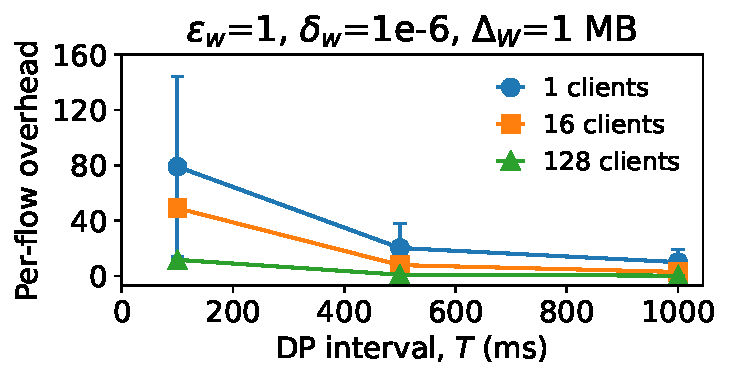
\includegraphics[width=\textwidth]{plots/overhead_vs_dp_interval_video.pdf}
      \caption{BW overhead vs DP interval (video)}
      \label{fig:video-overhead-vs-dpInt}
  \end{subfigure}
  \hfill
  \begin{subfigure}{0.49\columnwidth}
      \centering
      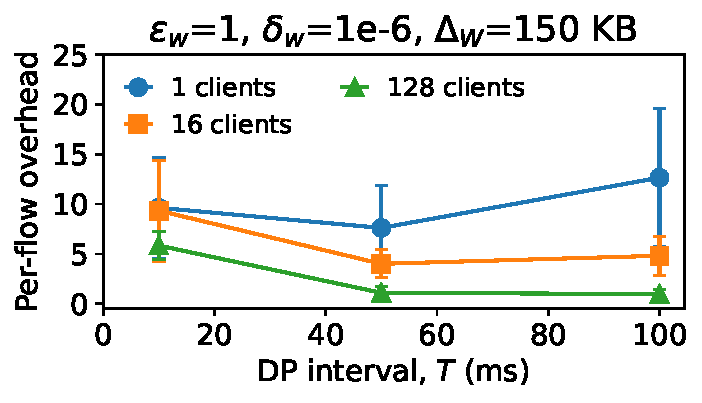
\includegraphics[width=\textwidth]{plots/overhead_vs_dp_interval_web.pdf}
      \caption{BW overhead vs DP interval (Web)}
      \label{fig:web-overhead-vs-dpInt}
  \end{subfigure}
  \caption{Video Streaming and Web Service; Bandwidth overhead for different values of DP interval.
  }
\end{figure}


\begin{figure}[t]
  \centering
  \begin{subfigure}{0.49\columnwidth}
      \centering
      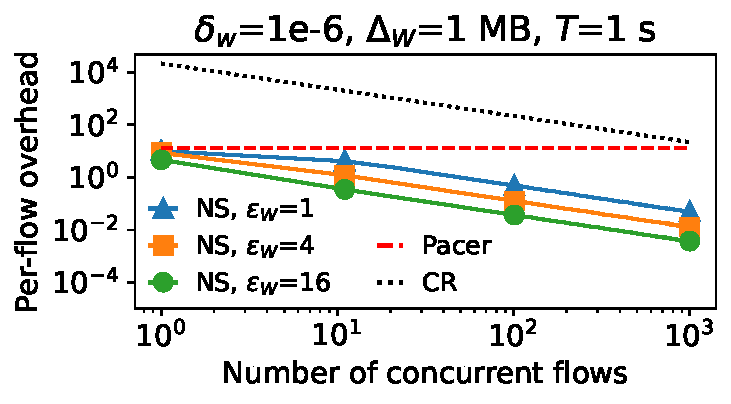
\includegraphics[width=\textwidth]{plots/overhead_vs_number_of_traces_video_loglog.pdf}
      \caption{Video streaming.}
      \label{fig:video-overheads-compare}
  \end{subfigure}
  \hfill
  \begin{subfigure}{0.49\columnwidth}
      \centering
      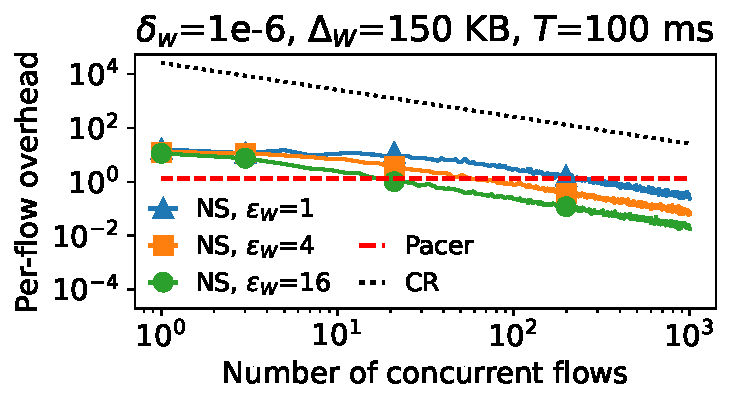
\includegraphics[width=\textwidth]{plots/overhead_vs_number_of_traces_web_loglog.pdf}
      \caption{Web service.}
      \label{fig:web-overheads-compare}
  \end{subfigure}
  \caption{Relative bandwidth overheads of {\sys} ({\ns}), constant
      shaping ({\constshape}), and Pacer.
  }
\end{figure}


\paragraph{Bandwidth overhead.}
\Cref{fig:video-overhead-vs-dpInt} shows the average per-flow relative bandwidth overhead as a function of different intervals and for varying number of clients.
The relative bandwidth overhead of a video is the number of dummy bytes transmitted normalized to the size of the unshaped video stream.
The error bars show the standard deviation in latency and bandwidth overhead.
We observe that the relative overhead decreases with larger values of $\dpintvl$.
While our simulation does not allow for the direct measurement of end-to-end latency, it's important to note that larger values for $\dpintvl$ result in data transmission occurring at more extended intervals, which can contribute to increased latency.
Therefore, the results show the trade-off between latency and bandwidth. 
A larger DP measurement interval implies higher download latency but fewer measurements and lower noise added to the payload, thus yielding a lower bandwidth overhead.
Thirdly, with multiple concurrent streaming clients, the bandwidth overhead is amortized.
Overall, {\sys}'s shaping can secure video streams with low bandwidth overheads.


\paragraph{Comparison with other techniques.}
\Cref{fig:video-overheads-compare} shows the per-flow relative bandwidth overhead of {\sys} ({\ns}) for video streaming application for varying with number of concurrent flows and for different values of $\varepsilon_{\winlen}$.
Except $\varepsilon_{\winlen}$, we use the same of parameters that we proposed in the beginning of this section.
We also compare with the overheads~that would be incurred due to constant rate
shaping ({\constshape}) and~Pacer \cite{mehta2022pacer} (see \Cref{subsubsec:background-defenses-pacer}), a SOTA system
that traffic shaping on a per-client request basis.

For {\constshape}, we configure the peak load for video service corresponding to
transmitting 1.7MB in every 5s, which is corresponding to transmitting the largest segment size in our video dataset. In other words, the {\constshape} mechanism always sends data at the maximum rate required to send a segment in our dataset.
In Pacer, for video service, we pad a segment at $i$\textsuperscript{th} index
in a video stream to the largest segment size at that index across all videos in the dataset. 
Even with the lowest privacy loss, $\varepsilon_{winlen}=1$, {\ns} add the same level of overhead as Pacer and 3 orders of magnitude less overhead than {\constshape}.  
Besides that, {\ns} can further amortize its overheads
among multiple concurrent streams within the tunnel without compromising privacy.





\subsection{Case Study: Web Service}\label{subsec:eval-bw-web}
In this section, we examine the effect of different privacy settings on bandwidth overhead for a web service.
We   
As we mentioned, we expect the values of DP measurement interval affects the communication end-to-end latency.
We choose smaller values for $\dpintvl$ for web service as compared to video streaming applications as web applications are delay-sensitive.
For the server responses, we use three values for DP measurement intervals, $\dpintvl$: 10 ms, 50 ms, 100 ms, and configure other parameters as follows: $\ssens = 150 KB$, $\winlen = 1s$, and
$\varepsilon_{\winlen} = 1$.
For the client requests, we use $\ssens = 200 B$, $winlen = 1s$, and $\varepsilon_{\winlen} = 1$.
We run experiments with 1, 16, and 128 video clients; each client requests a random webpage from the dataset.



\paragraph{Bandwidth overhead.}
\Cref{fig:web-overhead-vs-dpInt} shows the average per-web page relative bandwidth overhead, across all web page requests.
The bandwidth overhead for web traffic first reduces with increasing DP measurement interval from 10ms to 50ms, but interestingly, it increases again
with an interval of 100ms.
This is because, for small web pages, the DP interval of 100ms is larger than the total time required to download web pages.
As a result, additional overhead is incurred due to the padding of traffic in the 100ms intervals.
Similar to video streaming applications, when there are multiple concurrent requests from clients, the relative bandwidth overhead tends to decrease.

\paragraph{Comparison with other techniques.}
\Cref{fig:web-overheads-compare} shows the per-flow relative bandwidth overhead of {\sys} ({\ns}) for a web service for varying with number of concurrent flows and for different values of $\varepsilon_{\winlen}$.
We maintain the remaining parameters at the same values as previously mentioned.
Similar to video streaming, for web service, we compare {\sys} ({\ns}) with Pacer and constant rate shaping ({\constshape}).
For {\constshape}, we configure the peak load for web service corresponding to
transmitting 57KB in every 50ms, which is corresponding to transmitting the largest web page in our dataset.
For web services, Pacer pads all web pages to the largest page size, which is 147KB in our dataset.
Similar to video streaming case study, {\ns} introduces overheads that are several orders of magnitude smaller when compared to {\constshape}.
However,{\ns} requires more than 20 flows to achieve lower overhead than Pacer.
Pacer shapes server traffic only upon receiving a client request and does not
shape client traffic. 
Thus, it leaks the timing and shape of client requests, which could potentially reveal information about the server responses \cite{chen2010reality}.
{\sys} shapes traffic in both directions, which incurs higher overhead at the cost of stronger privacy than Pacer. 